\documentclass{article}
\usepackage{soul}
\usepackage[utf8]{inputenc}
\usepackage{xcolor}  % 用于颜色改变
\sethlcolor{yellow}  % 设置highlight的颜色为红色,如果需要黄色则改回yellow
\usepackage{amsmath}
\usepackage{amssymb}
\usepackage{amsfonts}
\usepackage{mathabx}
\usepackage{cancel}
\usepackage{graphicx}
\usepackage{tikz}

\title{MATH2022}
\author{Usyd Mingyuan Ba}
\date{\today}

\begin{document}

\maketitle

\section{Week1}
%================================================================================
\subsection{Arithmetics} % 修正使用 \subsection 或其他适当命令
\begin{itemize}

\item Addition \\
Operations Used: $+,\times$ \\
Limits: $-,/$ 

\item Integers \\
Operations Used: $+,\times,-$ \\
Limits: $/$ 

\item The Rational Numbers  \\
$\mathbb{Q} = \{\frac{p}{q} \mid p,q \in \mathbb{Z}, q \neq 0\}$\\
Operations Used: $+,-,\times,/$ \\
Limits: 

\item The Real Numbers  \\
Operations Used: $+,-,\times,/$ \\
Limits: $i = \sqrt{-1}$ 

\item The Complex Number  \\
$\mathbb{C} = \{a+bi \mid a,b\in \mathbb{R} where i = \sqrt{-1}\}$
Operations Used: $+,-,\times,/$ \\
Limits: 

\item Modular Arithmetic  \\
Let $n \in \mathbb{Z^{*}}$ and let $Z_n$ be the set
of remainders after dividing by n.\\
So $Z_n = \{0,1,2,3 ... n-1\}$

\end{itemize}


%================================================================================
\subsection{Fields}

A \textbf{field} $(F, +, \cdot)$ is a set $F$ equipped with two operations: addition ($+$) and multiplication ($\cdot$), satisfying the following axioms:

\begin{enumerate}
    \item \textit{Closure under Addition and Multiplication}
    \begin{align*}
        \forall a, b \in F, \quad & a + b \in F \\
        \forall a, b \in F, \quad & a \cdot b \in F
    \end{align*}
    
    \item \textit{Associativity of Addition and Multiplication}
    \begin{align*}
        \forall a, b, c \in F, \quad & (a + b) + c = a + (b + c) \\
        \forall a, b, c \in F, \quad & (a \cdot b) \cdot c = a \cdot (b \cdot c)
    \end{align*}
    
    \item \textit{Commutativity of Addition and Multiplication}
    \begin{align*}
        \forall a, b \in F, \quad & a + b = b + a \\
        \forall a, b \in F, \quad & a \cdot b = b \cdot a
    \end{align*}
    
    \item \textit{Identity Elements}
    \begin{align*}
        \exists 0 \in F \, \text{such that} \, \forall a \in F, \quad & a + 0 = a \\
        \exists 1 \in F \, \text{with} \, 1 \neq 0, \, \text{such that} \, \forall a \in F, \quad & a \cdot 1 = a
    \end{align*}
    
    \item \textit{Additive and Multiplicative Inverses}
    \begin{align*}
        \forall a \in F, \quad & \exists -a \in F \, \text{such that} \, a + (-a) = 0 \\
        \forall a \in F \, \text{with} \, a \neq 0, \quad & \exists a^{-1} \in F \, \text{such that} \, a \cdot a^{-1} = 1
    \end{align*}
    
    \item \textit{Distributivity of Multiplication over Addition}
    \begin{align*}
        \forall a, b, c \in F, \quad & a \cdot (b + c) = (a \cdot b) + (a \cdot c)
    \end{align*}
\end{enumerate}

%================================================================================



\subsection{Group Definition}

A \textbf{group} $(G, *)$ is a set $G$ together with a binary operation $*$ that combines any two elements $a$ and $b$ to form another element $a * b$. The binary operation satisfies the following four properties:

\begin{enumerate}
    \item \textit{Closure}: For every $a, b \in G$, the result of the operation $a * b$ is also in $G$.
    \[
    \forall a, b \in G, \quad a * b \in G
    \]

    \item \textit{Associativity}: For every $a, b, and c \in G$, the equation $(a * b) * c = a * (b * c)$ holds.
    \[
    \forall a, b, c \in G, \quad (a * b) * c = a * (b * c)
    \]

    \item\textit{Identity Element}: There exists an element $e \in G$, called the identity element, such that for every element $a \in G$, the equation $e * a = a * e = a$ holds.
    \[
    \exists e \in G \text{ such that } \forall a \in G, \quad e * a = a * e = a
    \]

    \item \textit{Inverse Element}: For each $a \in G$, there exists an element $b \in G$ such that $a * b = b * a = e$, where $e$ is the identity element.
    \[
    \forall a \in G, \quad \exists b \in G \text{ such that } a * b = b * a = e
    \]
\end{enumerate}

A group is called \textbf{abelian} (or \textbf{commutative}) if, in addition, the binary operation is commutative, that is, $a * b = b * a$ for all $a, b \in G$.\\

\textbf{Notes:}
\begin{enumerate}
\item As in the case of fields, the identity element and the inverse can be shown to be unique.
\item Our notation might imply that this operation is multiplication, but it could just as easily be addition or
another operation.
\end{enumerate}


%================================================================================
\subsection{Cyclic Groups}

A \textbf{cyclic group} $G$ is a special type of group that can be entirely generated by a single element $g \in G$. This element $g$ is called a generator of the group. The main characteristic that distinguishes cyclic groups from general groups is the ability to generate all elements of the group by repeatedly applying the group operation to the generator.

\begin{enumerate}
    \item \textit{Generator}
    \begin{align*}
        \exists g \in G \, \text{such that} \, G = \{g^n | n \in \mathbb{Z}\} \, \text{(for multiplicative groups)} \\
        \text{or} \quad G = \{ng | n \in \mathbb{Z}\} \, \text{(for additive groups)}
    \end{align*}
    
    \item \textit{Uniqueness}
    \begin{align*}
        \text{Every element of } G \text{ can be uniquely expressed as } g^n \text{ for some } n \in \mathbb{Z}.
    \end{align*}
\end{enumerate}

The cyclic nature of $G$ implies that it possesses a structure that can be systematically described by the powers (or multiples) of a single element, making cyclic groups particularly simple to understand and work with.

%================================================================================
\newpage
%================================================================================

\subsection{Symmetric Groups}

A \textbf{symmetric group} $S_n$ on a set of $n$ symbols is the group consisting of all possible permutations of these symbols, with group operation being the composition of these permutations. The symmetric group on $n$ symbols is denoted as $S_n$ and plays a crucial role in various areas of mathematics due to its fundamental nature in the study of permutations.\\

\begin{enumerate}
    \item \textbf{Recap}\\
    \textit{definitions}: A bijection is a mapping that is injective (one to one) and surjective (onto). \\

    \hl{\textit{Important Convention}}\\
    We write the action of $f: X \rightarrow Y$ on the right:
    \begin{center}
        $x \mapsto xf$ $(\forall x \in X)$
    \end{center}
    and we compose from left to right:
    \begin{center}
        $fg: X \rightarrow Z$ (where $f:X \rightarrow Y$,
        $g:Y \rightarrow Z$)
    \end{center}
    Instead of using $f \circ g(x) = f(g(x))$, we use $x(fg) := (xf)g$\\
    \textit{We apply f on x first, then g}

    \item Proof that: \textit{The composite of two bijection is also a bijection}\\
    Let $f: X \rightarrow Y, g: Y \rightarrow Z$
    \begin{itemize}
        \item Injective: Need to show that if $x(fg)=y(fg)$ then $x=y$\\
        Suppose $x(fg)=y(fg)$.Then $(xf)g = (yf)g$ by definition,So $xf =yf$ since g is injective,samething agagin, x = y.\\

        \item Surjective: Need to show that the range of $x(fg)$ equals to $Z$
    \end{itemize} 


    \item \textbf{Permutations}
    \begin{itemize}
        \item For a finite set of size n, there are \hl{n!} permutations (write $|X|=n$ ), The set of permutations of X is denoted $Sym(X)$ or $S_x$,So,\hl{$|Sym(X)|=n!$}
    \end{itemize}

    \item \hl{THEOREM}: \\
    The set of permutations on a set X, Sym(X), is a group under composition of permutations. We call it the Symmetric Group on X:

    \begin{itemize}
        \item \textbf{closure} The composite of two bijections is also a bijection.
        \item \textbf{associative} Composition of bijections is associative.
        \item \textbf{Identity element} The identity map is a bijection.
        \item \textbf{Inverse element} The inverse of a bijection is a bijection
    \end{itemize}  


\end{enumerate}

\section{Week2}

\section*{Week 3}

\subsection*{Matrix Recap}
\begin{itemize}
    \item \textbf{Elementary Matrices and Invertibility}
    \item \textbf{Determinants, Properties}
\end{itemize}

\subsection*{Odd and Even Permutations}
\begin{itemize}
    \item \textbf{Transposition}\\
    \textit{Definition}: A transposition is a permutation 
    $\phi: \mathbb{X} \rightarrow \mathbb{X}$, which interchanges two distinct elements $a,b \in \mathbb{X}$ leaving all other elements unchanged. Thus,
    \begin{center}
        $\phi = (ab)$.
    \end{center}
    
    \textit{Fact}: All \hl{cycles} are a product (composition) of transpositions.
    \begin{center}
        $(a_1,a_2,a_3, \ldots, a_n) = (a_1 a_2)(a_1a_3)\ldots(a_1a_n)$.
    \end{center}
    
    \textit{Corollary}: Every permutation of a finite set is a product (composition) of transpositions.
    
    \item \textbf{Even/Odd}\\
    \textit{Definition}: We call a permutation even (or odd) if it is a product of an even (or odd, respectively) number of transpositions.
    \begin{itemize}
        \item $(123) = (12)(13)$ is \hl{even}.
        \item $(1234) = (12)(13)(14)$ is \hl{odd}.
        \item $(1) = (12)(12) = (13)(13)$ is \hl{even}.
    \end{itemize}
    \textit{Properties}:
    \begin{itemize}
        \item Single transpositions are self-inverse: $(ab)(ab) = 1$.
        \item A permutation and its inverse have the same parity.
    \end{itemize}


    \item \textbf{Permutation Matrix}\\
    \textit{Definition}: A permutation matrix is the result of applying a permutation to the rows of the identity matrix.
    \begin{center}
        $\phi = (132) = (13)(12) = R_1 \leftrightarrow R_3, R_1 \leftrightarrow R_2$.
    \end{center}
    Hence, \hl{$\text{Det}(M) = \text{Det}(E_1 E_2) = \text{Det}(E_1)\text{Det}(E_2) = (-1)^2 = 1$}.

\end{itemize}
\newpage

\subsection*{The Alternating Subgroup, $\text{Alt}(n)$, of $\text{Sym}(n)$}

\begin{itemize}
    \item \textbf{Subgroup}\\
    \textit{Definition}: A subgroup, $H$, of a group, $G$, is a subset of $G$ which is also a group 
    under the same operation. We write $H \leq G$ or $H < G$ if $H$ is a proper subset of $G$.
    
    \textit{Proof a subgroup}:
    \begin{itemize}
        \item It is non-empty
        \item  It is closed under the operation.\\
        Associativity: Inherited from G\\
        Identity: $\exists a \in G, a^k = e$ \\
        Inverse: $a^k = e \rightarrow aa^{k-1} = e = a^{k-1}a$
    \end{itemize}



    \item \textbf{Alternating Group}\\
    \textit{Definition}: The alternating group (on \(n\) letters) is the set of even permutations 
    in \(Sym(n)\). That is, \(Alt(n) = \{\)even permutations of \(\{1, 2, \ldots, n\}\}\).
    \begin{figure}[htbp]
        \centering % 图片居中
        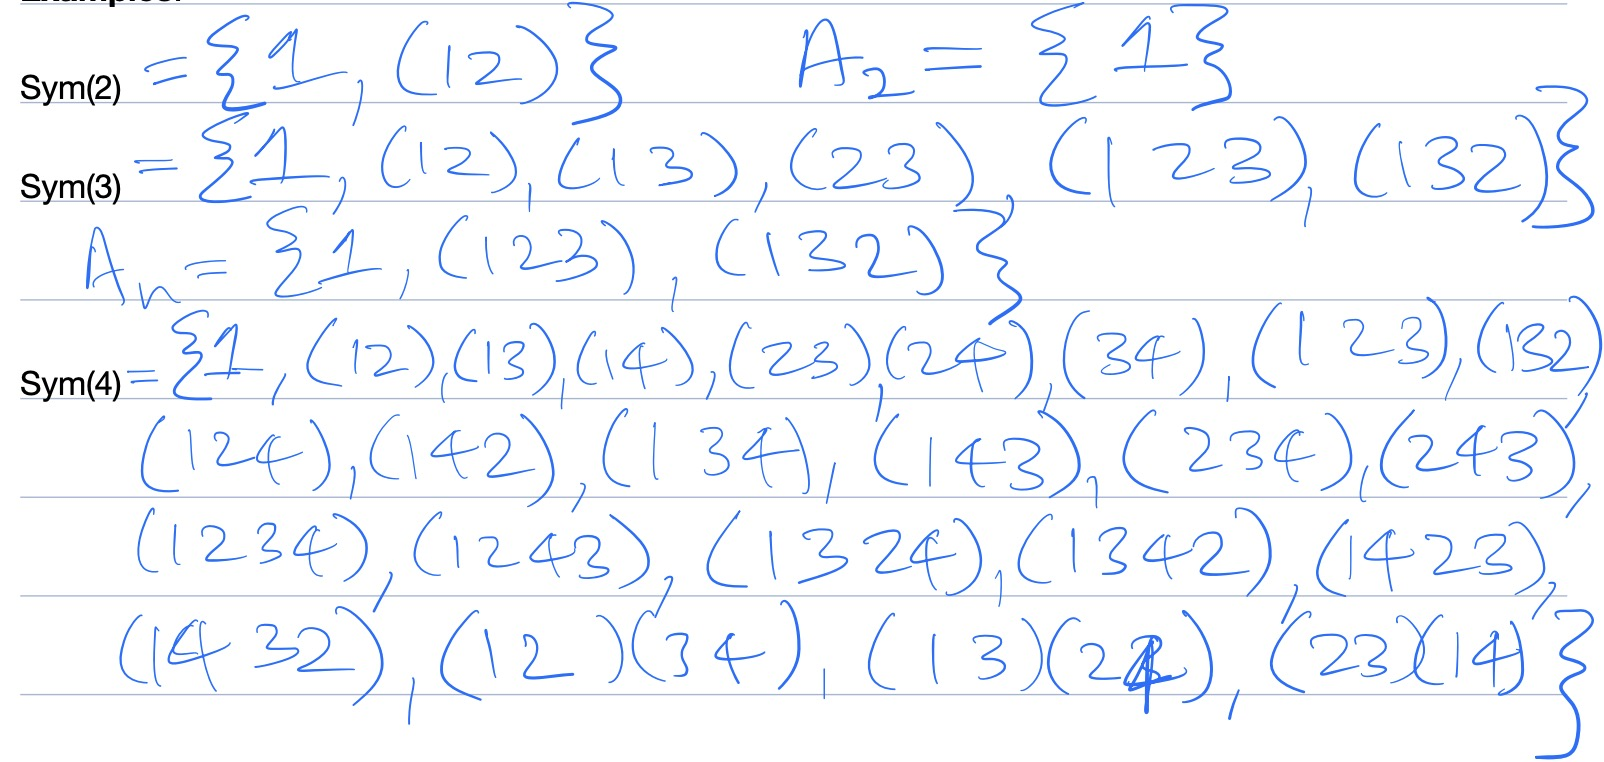
\includegraphics[width=1.0\textwidth]{Graphs/Alternative_Group.jpg} % 插入图片,并设置图片宽度为文本宽度的80%
    \end{figure}

\end{itemize}

\newpage

\section*{Week4}

\begin{enumerate}
    \item Elementary matrices: An $n \times n$ matrix is called elementary if it is the result of applying a single elementary row operation to the identity matrix $I_{n}$.
    \item Effect of multiplication by an elementary matrix: If $E$ is the elementary matrix obtained by applying the elementary row operation $\rho$ to $I_{n}$, and $A$ is any matrix with $n$ rows, then the matrix product $E A$ is the matrix obtained by applying $\rho$ to $A$.
    \item Invertibility criterion and algorithm: A square matrix $A$ is invertible if and only if $A$ is a product of elementary matrices, which occurs if and only if the augmented matrix $[A \mid I]$ can be row reduced to $[I \mid B]$, in which case $A^{-1}=B$.
    \item Half of the definition of invertibility suffices for square matrices: If $A$ is a square matrix and $A B=I$ or $B A=I$ then $A B=B A=I$, in which case the inverse $A^{-1}$ exists and equals $B$.
    \item Determinants of matrices of dimensions 1,2 and 3: The determinant of a $1 \times 1$ matrix $[a]$ is simply the entry $a$. The determinant of a $2 \times 2$ matrix $A=\left[\begin{array}{cc}a & b \\ c & d\end{array}\right]$ is $\det A=\left|\begin{array}{cc}a & b \\ c & d\end{array}\right|=a d-b c$. The determinant of a $3 \times 3$ matrix $A=\left[\begin{array}{ccc}a & b & c \\ d & e & f \\ g & h & k\end{array}\right]$ is
    \[
    \det A=|A|=a\left|\begin{array}{cc}
    e & f \\
    h & k
    \end{array}\right|-b\left|\begin{array}{cc}
    d & f \\
    g & k
    \end{array}\right|+c\left|\begin{array}{cc}
    d & e \\
    g & h
    \end{array}\right|
    \]
    called the expansion along the first row, where the smaller determinant arises by ignoring the row and column of the entry being used as a coefficient.
    \item Determinants in general: Following the pattern for $3 \times 3$ matrices, we may expand along any row or down any column of a given square matrix $A$ of any size, producing the same number, called the determinant of $A$, denoted by $\det A$ or $|A|$, provided one uses adjustment factors given by the chequerboard patterns
    \[
    \left[\begin{array}{ccc}
    + & - & + \\
    - & + & - \\
    + & - & +
    \end{array}\right], \quad\left[\begin{array}{cccc}
    + & - & + & - \\
    - & + & - & + \\
    + & - & + & - \\
    - & + & - & +
    \end{array}\right]
    \]
    and so on to higher dimensions.
    \item Multiplicative property of determinants: If $A$ and $B$ are square matrices of the same size then $\det(A B)=(\det A)(\det B)$.
    \item Invertibility criterion using determinants: A square matrix is invertible if and only if its determinant is nonzero.
    \item Effects of elementary row and columns operations on determinants: Let $A$ be a square matrix. If $B$ is obtained from $A$ by swapping two rows or swapping two columns then
    \[
    \det B=-\det A \text{.}
    \]
    If $B$ is obtained from $A$ by multiplying a row or column by a scalar $\lambda$ then
    \[
    \det B=\lambda \det A \text{.}
    \]
    If $B$ is obtained from $A$ by adding a multiple of one row [column] to another row [column] then
    \[
    \det B=\det A \text{.}
    \]
    \item Determinant of the transpose: If $A$ is a square matrix then $\det\left(A^{T}\right)=\det A$.
    \item Transpositions: A permutation that interchanges two letters and fixes all other letters is called a transposition.
    \item \hl{Even and odd permutations:} A permutation of a finite set is called even if it is a product of an even number of transpositions (and by default the identity permutation is even), and called odd if it is a product of an odd number of transpositions.
    \item \hl{No permutation can be both even and odd:} If $n$ is a positive integer then the symmetric group $S_{n}$ is the disjoint union of $A_{n}$, the subset of even permutations (and called the alternating group), and $S_{n} \backslash A_{n}$, the complement of $A_{n}$, which comprises exactly the subset of all odd permutations.
    
    \newpage

    \item \hl{Cosest}:For a Symmetric Group $S_n, n\geq 2$,
    \begin{itemize}
        \item \textbf{Symmetric Group and Cosets:} The symmetric group, denoted as $S_n$, represents the group of all permutations of $n$ elements. Within this group, a \textit{coset} is a form of subset created by multiplying a group element by every element within a subgroup. Specifically, for a subgroup $H$ in a group $G$, and any element $g \in G$, we define:
        \begin{itemize}
            \item A \textit{left coset} of $H$ in $G$ with respect to $g$ as $gH = \{gh : h \in H\}$.
            \item A \textit{right coset} of $H$ in $G$ with respect to $g$ as $Hg = \{hg : h \in H\}$.
        \end{itemize}
        Important properties of cosets include:
        \begin{itemize}
            \item Cosets of a subgroup partition the group.
            \item All left (or right) cosets of a subgroup have the same cardinality as the subgroup itself.
        \end{itemize}
    \end{itemize}

    \begin{figure}[htbp]
        \centering % 图片居中
        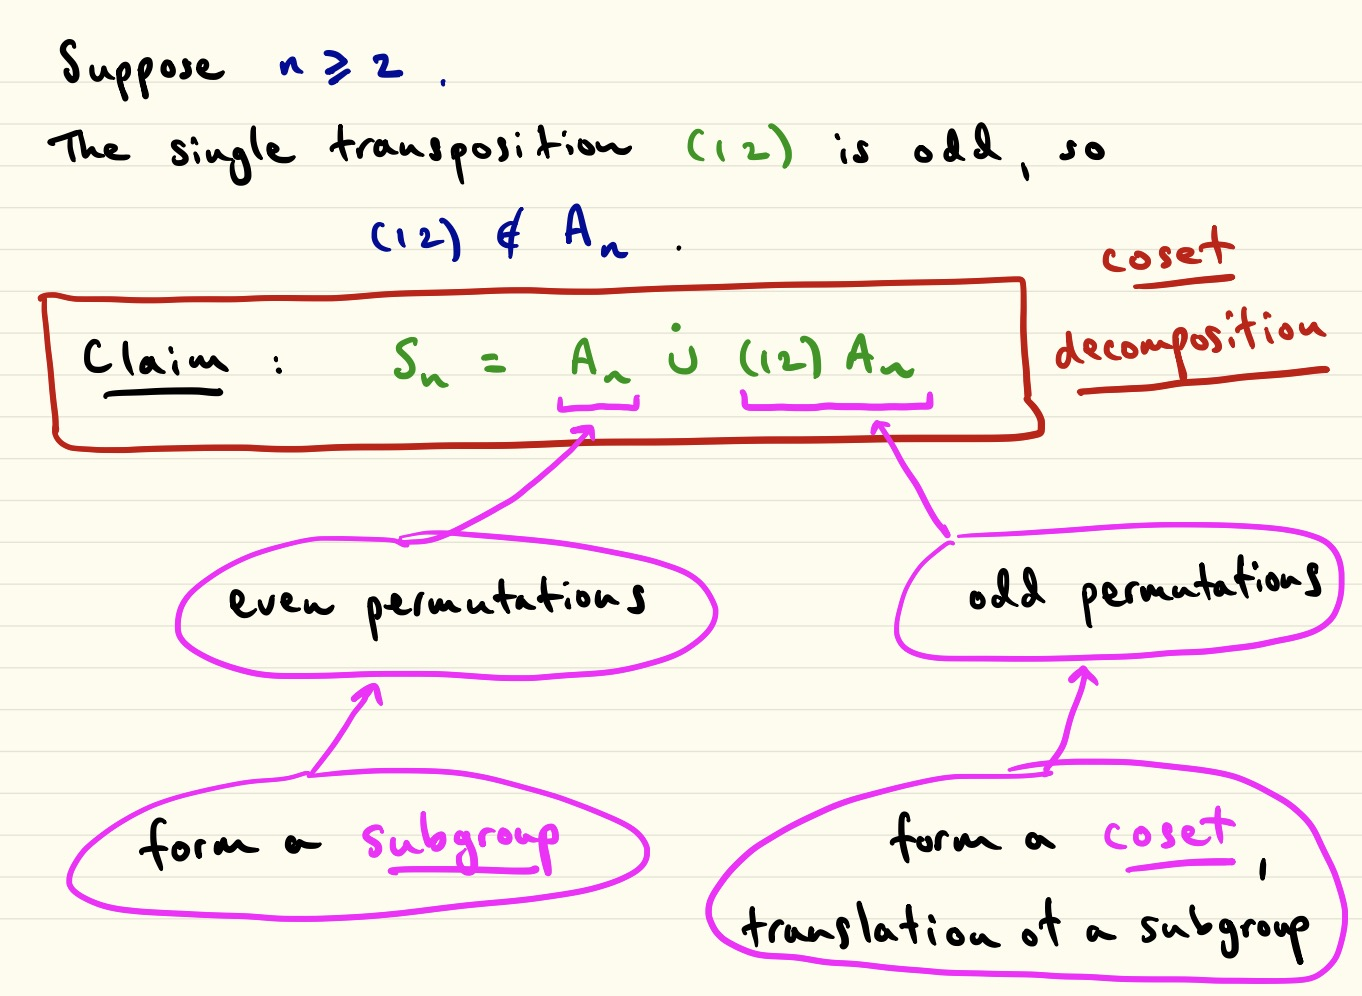
\includegraphics[width=0.8\textwidth]{Graphs/Coset.jpg} % 插入图片,并设置图片宽度为文本宽度的80%
    \end{figure}
    
    \newpage

    \item Conjugates of permutations: If $\alpha$ and $\beta$ are any permutations of a given set then the conjugate of $\alpha$ by $\beta$ is the permutation \hl{$\beta^{-1} \alpha \beta$}, denoted by $\alpha^{\beta}$, using exponential notation. We denote by $\alpha^{-\beta}$ the inverse of $\alpha^{\beta}$, so that $\alpha^{-\beta}=\beta^{-1} \alpha^{-1} \beta$, the conjugate of $\alpha^{-1}$ by $\beta$ (not to be confused with $\beta \alpha \beta^{-1}$, which is $\alpha^{\beta^{-1}}$, the conjugate of $\alpha$ by $\beta^{-1}$.
    \item \textbf{\textit{Properties on Conjugation:}}
            Let $(S,*)$ be a set with an associative binary operation, $*$ , and an identity element, e.
            \begin{itemize}
                \item \textit{multiplicative} $(ab)^c = a^{c}b^{c}$
                \begin{center}
                    $(ab)^c = c^{-1} (a b) c = (c^{-1} a c) (c^{-1} b c) = a^{c}b^{c}$
                \end{center}

                \item $(a^b)^{-1} = (a^{-1})^{b}$ \\
                \textit{Note that}: $a^{b^{-1}}$ is the conjugate of $a$ by $b^{-1}$ 
            \end{itemize}

    \item Effect of conjugation on the cycle decomposition of a permutation: If $\alpha$ and $\beta$ are permutations and $\left(\begin{array}{llll}a_{1} & a_{2} & \ldots & a_{k}\end{array}\right)$ is a cycle in the cycle decomposition of $\alpha$ then $\left(a_{1} \beta a_{2} \beta \ldots a_{k} \beta\right)$ is a cycle in the cycle decomposition of the conjugate $\alpha^{\beta}$.
    \item \textbf{\textit{More on Conjugation}}: \\Suppose $\alpha,\beta \in Sym(n)$,we want to write decomposition of $\alpha^{\beta}$
    from the cycle decomposition of $\alpha$.
    \begin{itemize}
        \item \hl{Lemma}:If $(a_1,a_2,a_3 ...... a_k)$ is cycle in $\alpha$,
        then $(a_1\beta a_2\beta a_3\beta a_4\beta ... a_k\beta)$ is a cycle in $\alpha^{\beta}$.(\hl{$a_k \beta$ means $\beta(a_k)$})
        \\\\\textbf{\textit{Proof}}
        \begin{center}
            Suppose $i \in \{1,2,3 ... k-1\}$,Then\\
            $(a_i \beta) \rightarrow (a_i \beta)(\beta^{-1}a \beta) = a_i \beta \beta^{-1} a \beta
            = a_i a \beta = a_{i+1} \beta$
        \end{center}
        Similarly
        \begin{center}
            $(a_k \beta) \rightarrow (a_k \beta)(\beta^{-1}a \beta) = a_k \beta \beta^{-1} a \beta
            = a_k a \beta = a_1 \beta$
        \end{center}
        \hl{$\rightarrow$} stands for "maps to".
        \\\hl{This proof only shows that the conjugate of a cycle is in(one of) $\alpha^{\beta}$. }
        But in fact:
        \begin{center}
            $(a_1a_2a_3...a_k)^{\beta} = (a_1\beta a_1\beta ... a_k\beta) (\star)$
        \end{center}
        Which means the conjugate of a cycle $a_i$ is exactly a $a_i \beta$.
    \item \textbf{\textit{Corollary}}: To find $\alpha^{\beta}$, just replace every $a_i$, in each cycle with $a_i \beta$
        \begin{center}
            \textbf{Proof}: If $\alpha = a_1 a_2 a_3... a_k$ for cycles $a_i$, 
            the conjugate $\alpha ^{\beta} = a_1 ^{\beta} a_2 ^{\beta} a_2 ^{\beta} ... a_k ^{\beta}$ ------ \textit{multiplicativity}
            \\$= (a_1\beta a_1\beta ... a_k\beta)$ ------ \textit{see $\star$ above}

        \end{center}
    
    \end{itemize}
\end{enumerate}


\end{document}
